\documentclass[../index.tex]{subfiles}

\begin{document}
    % 2.1
    \section{Khảo sát hiện trạng}
    % 2.1.1
    \subsection{Xác định yêu cầu chức năng}
    Hệ thống cần xử lý được một số các chức năng sau:
    \begin{itemize}
        \item Chức năng đăng nhập, đăng ký, quên mật khẩu.

        \item Chức năng xem thông tin người dùng, cập nhật thông tin cá nhân.

        \item Chức năng xem bài viết, đăng bài, bình luận, tạo bình luận, bỏ phiếu
            và báo cáo bài viết.

        \item Chức năng quản lý trò chuyện.

        \item Chức năng quản lý thông báo.

        \item Chức năng quản lý diễn đàn, chủ đề.

        \item Chức năng quản lý thành viên.

        \item Chức năng quản lý vai trò và phân quyền động.

        \item Chức năng thống kê.
    \end{itemize}
    % 2.1.1
    \subsection{Xác định yêu cầu phi chức năng}
    \begin{table}[H]
        \centering
        {}
        \begin{tabular}{|p{2cm}|p{5cm}|p{7cm}|}
            \hline
            Yêu cầu              & Mô tả                                                               & Ví dụ                                                                                                   \\
            \hline
            Môi trường           & Môi trường hoạt động của hệ thống                                   & Hoạt động ổn định hầu hết các trình duyệt hiện nay                                                      \\
            \hline
            Xác thực và ủy quyền & Các cơ chế xác thực, cơ chế phân quyền mạnh mẽ                      & Xác thực sử dụng JWT, và áp dụng RBAC cho cơ chế ủy quyền                                               \\
            \hline
            Hiệu năng            & Tốc độ phản hồi nhanh chóng, có khả năng mở rộng, khả năng chịu tải & Diễn đàn cần phản hồi nhanh chóng như tải trang, đăng bài, bình luận, tin nhắn, thông báo và upload ảnh \\
            \hline
            Giao diện            & Giao diện thân thiện, dễ sử dụng, phù hợp nhiều đối tượng           & Sử dụng các thiết kế hiện đại, theo xu hướng hiện nay, màu sắc bắt mắt                                  \\
            \hline
        \end{tabular}
        \caption{Yêu cầu phi chức năng của hệ thống}
    \end{table}
    Các yêu cầu phi chức năng đóng vai trò quan trọng trong việc đảm bảo chất
    lượng và thành công của một hệ thống. Bằng cách xác định rõ và đánh giá các yêu
    cầu này, chúng ta có thể xây dựng một hệ thống đáp ứng được nhu cầu của
    người dùng và đạt được các mục tiêu nghiệp vụ.

    % 2.2
    \section{Biểu đồ Use Case}
    
    \subsection{Biểu đồ Use Case tổng quát}
    \begin{figure}[H]
        \centering
        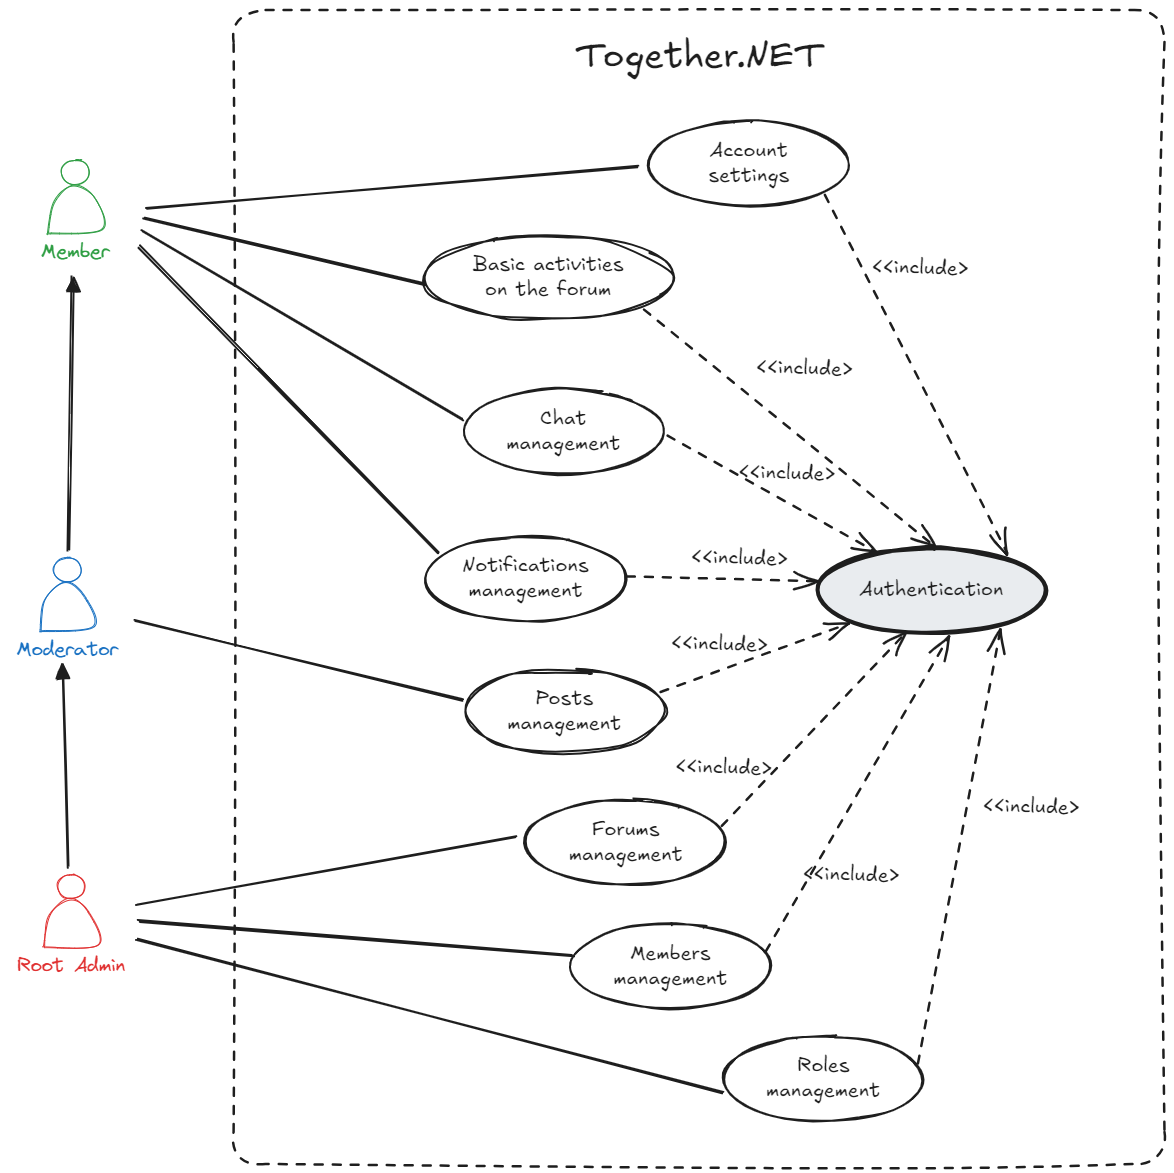
\includegraphics[width=0.85\linewidth]{../figures/usecase-summary.png}
        \caption{Biểu đồ Use Case tổng quát}
    \end{figure}
    Biểu đồ Use Case tổng quát trên mô tả các tương tác giữa các tác nhân và hệ
    thống. Hệ thống này có 3 loại tác nhân chính:
    \begin{enumerate}
        \item \textbf{Member}: Là thành viên thông thường của hệ thống, có thể
            thực hiện các hoạt động như tạo tài khoản, cập nhật thông tin cá nhân,
            đăng bài, bình luận, vote cho bài viết và nhận thông báo.

        \item \textbf{Moderator}: Là người kiểm duyệt, có quyền hạn cao hơn
            Member. Ngoài các chức năng của Member, Moderator còn có thể quản lý
            các bài viết, bình luận, thông báo, và xử lý các trường hợp vi phạm.

        \item \textbf{Root Admin}: Là quản trị viên hệ thống, có quyền truy cập
            và điều khiển toàn bộ hệ thống. Root Admin có thể quản lý tất cả các
            chức năng của hệ thống, bao gồm quản lý thành viên, quản lý vai trò,
            và cấu hình hệ thống.
    \end{enumerate}
    Biểu đồ Use Case tổng quát trên cho thấy hệ thống có cấu trúc rõ ràng, phân chia
    quyền hạn giữa các loại tác nhân, và đáp ứng được các yêu cầu cơ bản của một
    hệ thống diễn đàn trực tuyến. Tuy nhiên, để có cái nhìn chi tiết hơn, chúng ta
    tiếp tục phân tích các biểu đồ usecase phân rã cụ thể.

    \subsection{Biểu đồ Use Case phân rã thông tin tài khoản}
    \begin{figure}[H]
        \centering
        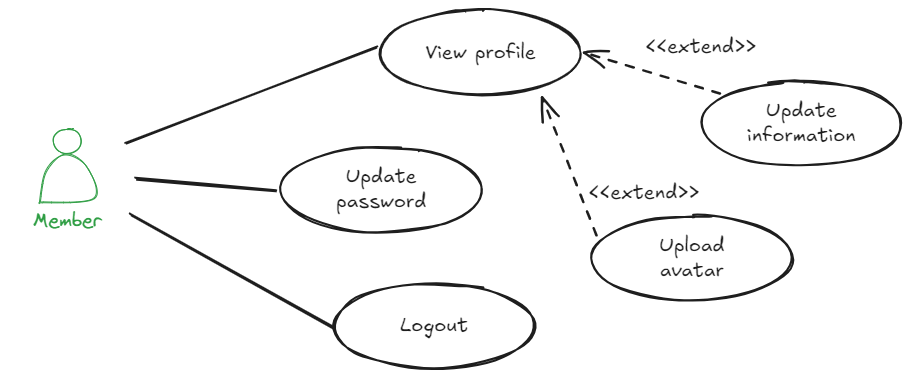
\includegraphics[width=0.85\linewidth]{
            figures/usecase-account-setting.png
        }
        \caption{Biểu đồ Use Case phân rã thông tin tài khoản}
    \end{figure}
    Các chức năng của mọi người dùng, bao gồm việc xem hồ sơ, cập nhật thông tin,
    thay đổi mật khẩu, tải lên ảnh đại diện, và đăng xuất. Các chức năng cập nhật
    thông tin và thay đổi mật khẩu được mở rộng từ chức năng xem hồ sơ.

    \subsection{Biểu đồ Use Case phân rã hoạt động cơ bản trên diễn đàn}
    \begin{figure}[H]
        \centering
        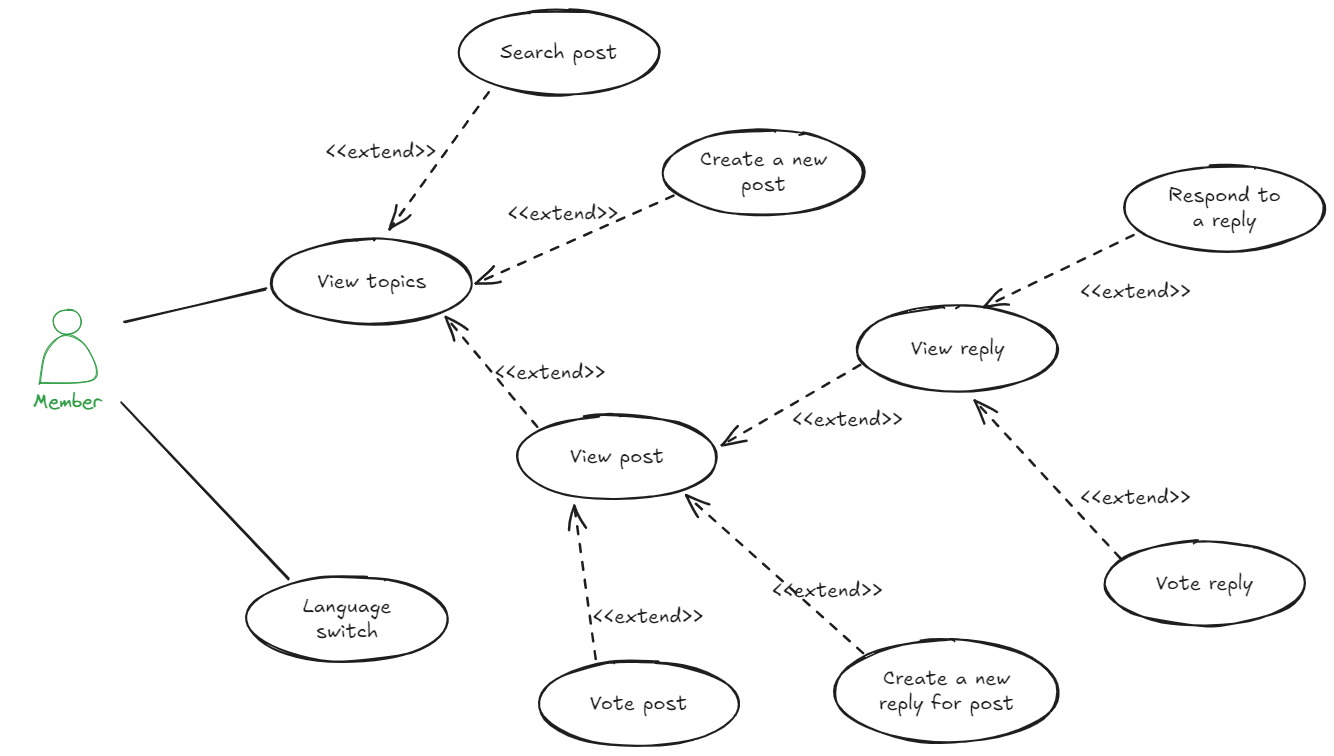
\includegraphics[width=0.85\linewidth]{
            figures/usecase-basic-activity.png
        }
        \caption{Biểu đồ Use Case phân rã hoạt động cơ bản trên diễn đàn}
    \end{figure}
    Các chức năng của thành viên, bao gồm việc xem các chủ đề, tìm kiếm bài viết,
    tạo bài viết mới, phản hồi bài viết, và bình chọn cho bài viết. Các chức năng
    như tạo bài viết, phản hồi, và bình chọn được mở rộng từ việc xem các chủ đề,
    cho phép người dùng tương tác và tham gia vào các cuộc thảo luận trên diễn
    đàn.

    \subsection{Biểu đồ Use Case phân rã quản lý chat}
    \begin{figure}[H]
        \centering
        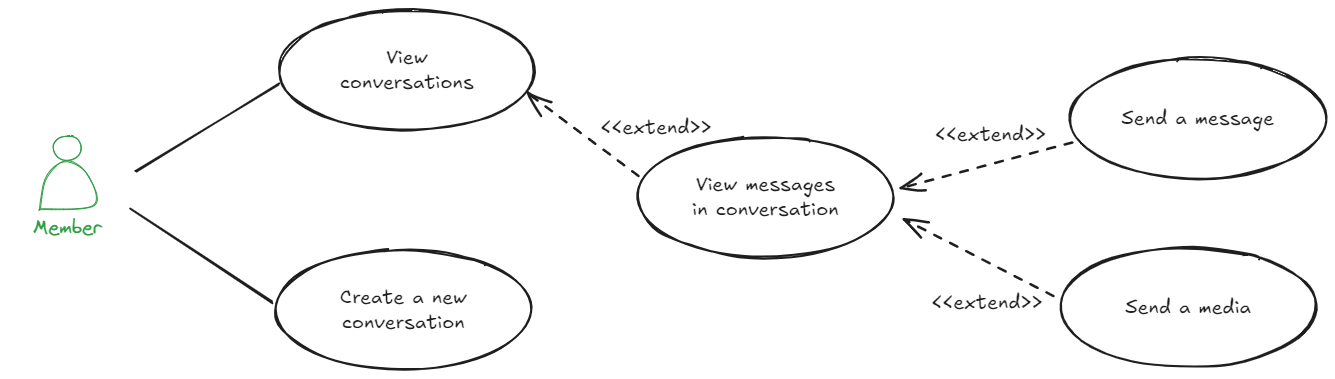
\includegraphics[width=0.85\linewidth]{
            figures/usecase-chat-management.png
        }
        \caption{Biểu đồ Use Case phân rã quản lý chat}
    \end{figure}
    Các chức năng chính trong hệ thống chat, bao gồm việc xem các cuộc trò chuyện,
    gửi tin nhắn và tạo cuộc trò chuyện mới. Thành viên có thể theo dõi các cuộc
    hội thoại, gửi tin nhắn trong các cuộc trò chuyện hiện có, và bắt đầu một cuộc
    trò chuyện mới với người khác, từ đó tạo điều kiện thuận lợi cho việc giao
    tiếp và kết nối giữa các thành viên.

    \subsection{Biểu đồ Use Case phân rã quản lý thông báo}
    \begin{figure}[H]
        \centering
        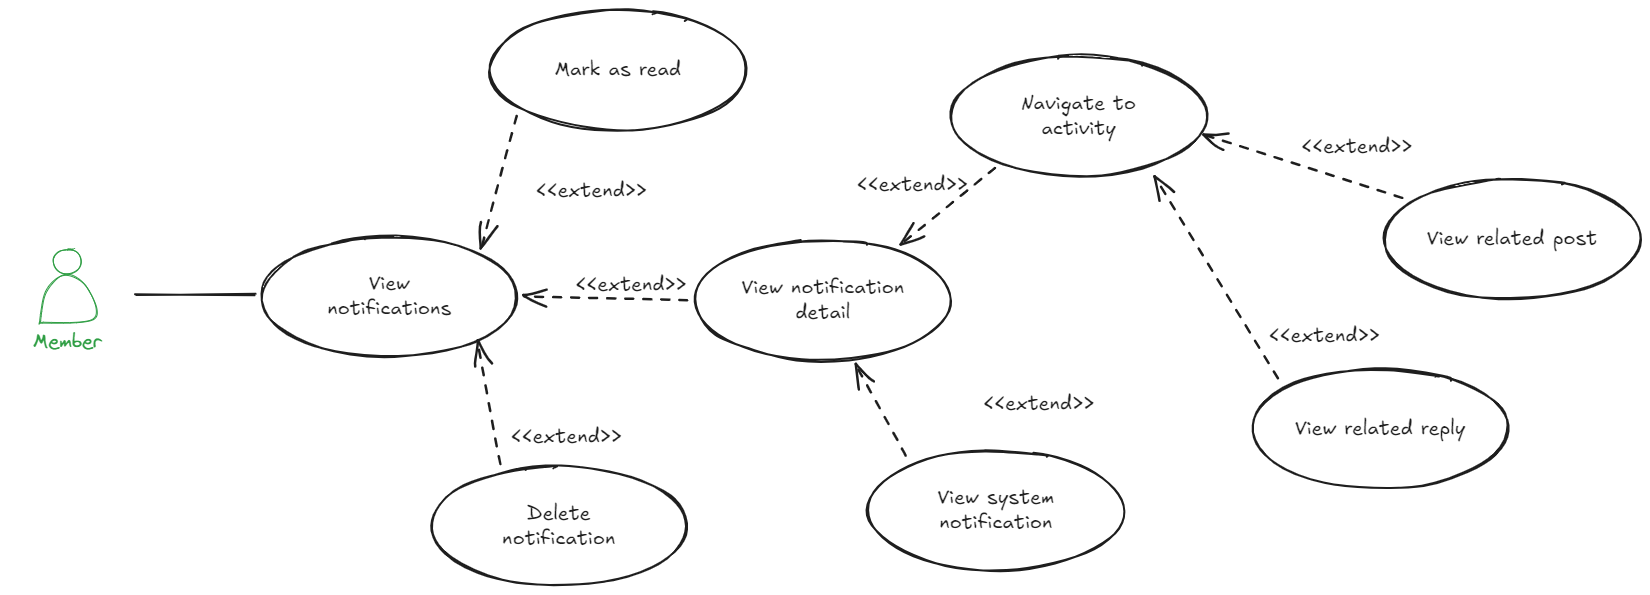
\includegraphics[width=0.85\linewidth]{
            figures/usecase-notification-management.png
        }
        \caption{Biểu đồ Use Case phân rã quản lý thông báo}
    \end{figure}
    Các chức năng liên quan đến việc nhận và xử lý thông báo trong hệ thống. Thành
    viên có thể xem danh sách thông báo, đánh dấu thông báo là đã đọc, và xem chi
    tiết thông báo cụ thể. Bên cạnh đó, họ cũng có thể điều hướng đến các hoạt động
    hoặc nội dung liên quan đến thông báo đó. Những chức năng này giúp thành
    viên cập nhật thông tin và tương tác hiệu quả hơn với các hoạt động trong hệ
    thống.

    \subsection{Biểu đồ Use Case phân rã quản lý bài viết}
    \begin{figure}[H]
        \centering
        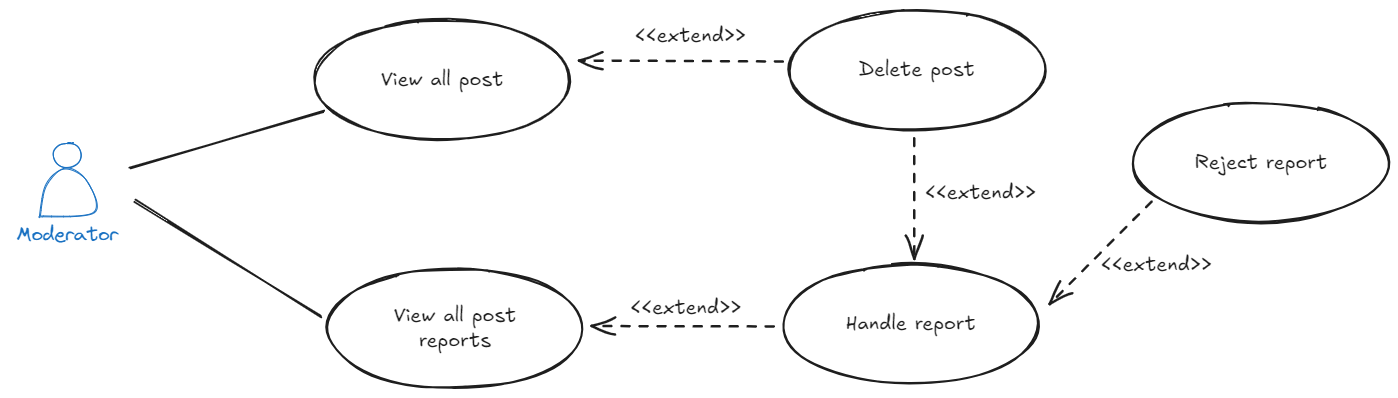
\includegraphics[width=0.85\linewidth]{
            figures/usecase-post-management.png
        }
        \caption{Biểu đồ Use Case phân rã quản lý bài viết}
    \end{figure}
    Các chức năng quản lý nội dung bài viết trong hệ thống. Người kiểm duyệt có thể
    xem toàn bộ bài viết, xóa các bài viết khi cần thiết, và xử lý các báo cáo liên
    quan đến bài viết. Ngoài ra, cũng có thể từ chối các báo cáo không hợp lệ.
    Những chức năng này giúp đảm bảo chất lượng nội dung và duy trì môi trường
    giao tiếp lành mạnh trong hệ thống.

    \subsection{Biểu đồ Use Case phân rã quản lý chủ đề}
    \begin{figure}[H]
        \centering
        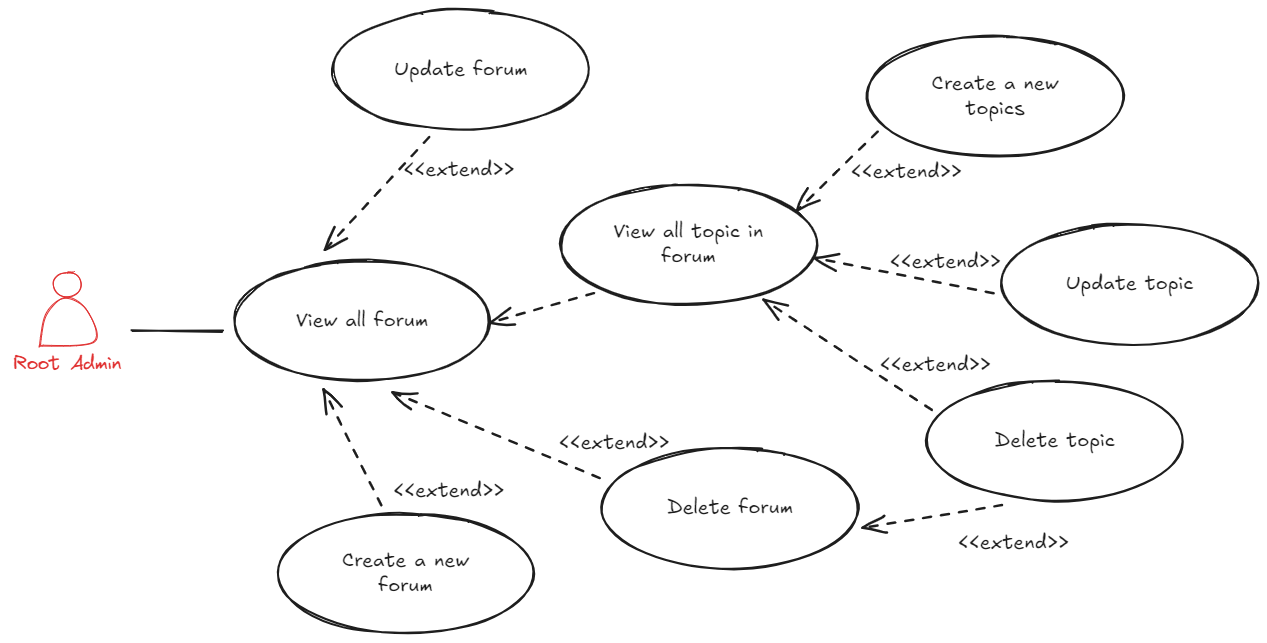
\includegraphics[width=0.85\linewidth]{
            figures/usecase-forum-management.png
        }
        \caption{Biểu đồ Use Case phân rã quản lý chủ đề}
    \end{figure}
    Quản trị viên có khả năng xem tất cả các diễn đàn, tạo diễn đàn mới, cập
    nhật thông tin của diễn đàn, và xóa những diễn đàn không còn cần thiết. Bên
    cạnh đó, cũng có thể tạo và cập nhật các chủ đề thảo luận, cũng như xóa các
    chủ đề không phù hợp. Những chức năng này giúp quản trị viên duy trì chất lượng
    và sự phong phú của nội dung trong hệ thống, đảm bảo rằng người dùng có trải
    nghiệm tốt nhất khi tham gia thảo luận.

    \subsection{Biểu đồ Use Case phân rã quản lý thành viên}
    \begin{figure}[H]
        \centering
        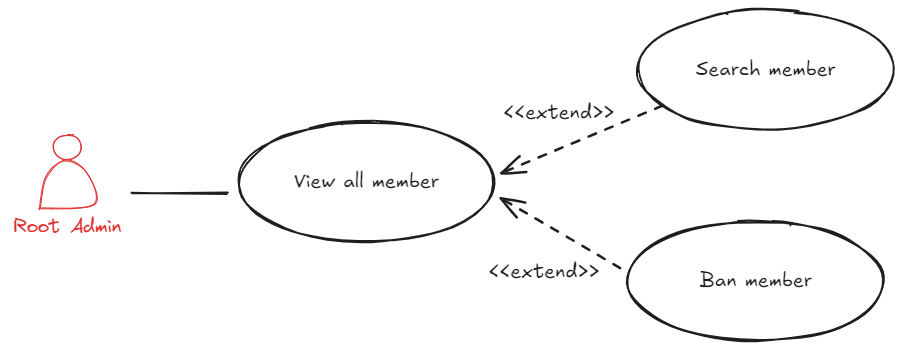
\includegraphics[width=0.85\linewidth]{
            figures/usecase-member-management.png
        }
        \caption{Biểu đồ Use Case phân rã quản lý thành viên}
    \end{figure}
    Các chức năng mà quản trị viên có thể thực hiện để quản lý các thành viên
    trong hệ thống. Quản trị viên có thể xem tất cả các thành viên và có thể tìm
    kiếm thành viên cụ thể để quản lý hiệu quả hơn. Nếu cần thiết, cũng có quyền
    cấm những thành viên vi phạm quy định của hệ thống. Những chức năng này giúp
    duy trì một môi trường giao tiếp lành mạnh và an toàn trong hệ thống, đảm bảo
    rằng các quy tắc được tuân thủ.

    \subsection{Biểu đồ Use Case phân rã quản lý vai trò}
    \begin{figure}[H]
        \centering
        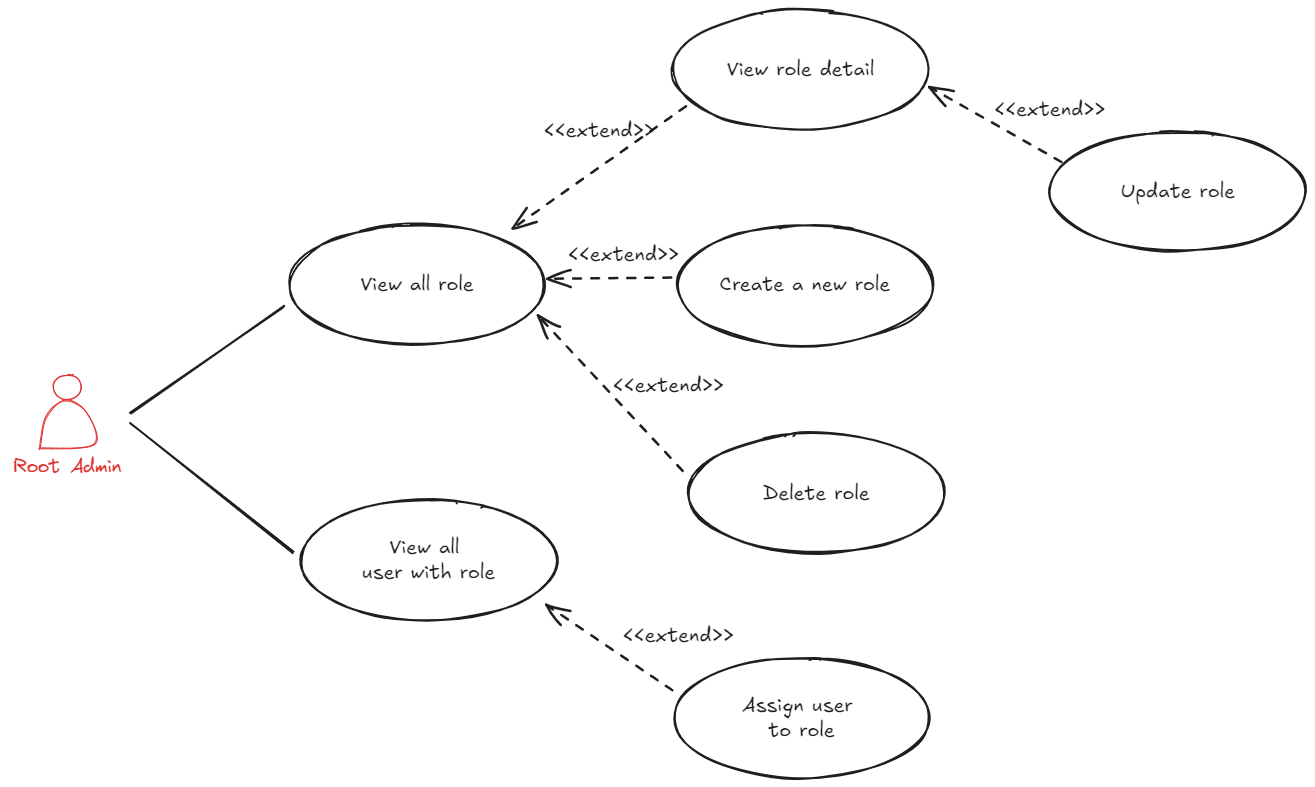
\includegraphics[width=0.85\linewidth]{
            figures/usecase-role-management.png
        }
        \caption{Biểu đồ Use Case phân rã quản lý vai trò}
    \end{figure}
    Quản trị viên có khả năng xem tất cả các vai trò hiện có, giúp họ nắm bắt
    cấu trúc quyền hạn trong hệ thống. Quản trị viên cũng có thể tạo vai trò mới
    để đáp ứng các nhu cầu quản lý khác nhau. Ngoài ra, có thể cập nhật thông tin
    của các vai trò hiện có hoặc xóa những vai trò không còn cần thiết. Quản trị
    cũng có thể xem tất cả người dùng và phân quyền cho họ dựa trên vai trò đã
    được thiết lập. Những chức năng này đảm bảo rằng hệ thống có tổ chức và các quyền
    hạn được phân bổ hợp lý, tạo điều kiện thuận lợi cho việc quản lý.

    % 2.3
    \section{Đặc tả chức năng}

    \subsection{Đặc tả Use Case Đăng nhập}
    \begin{table}[H]
        \centering
        {}
        \begin{tabular}{ |p{3cm}|p{9cm}| }
            \hline
            Usecase         & Đăng nhập                                                                                   \\
            \hline
            Mô tả           & Người dùng đăng nhập vào hệ thống để sử dụng các chức năng đã được hệ thống ủy quyền        \\
            \hline
            Actor           & Thành viên                                                                                  \\
            \hline
            Pre-Condition   & Tài khoản đã có trên hệ thống                                                               \\
            \hline
            Post-Condition  & Thông tin đăng nhập sẽ được hệ thống lưu lại                                                \\
            \hline
            Basic flows     & \begin{enumerate}
                \item Người dùng nhập thông tin đăng nhập
                \item Hệ thống kiểm tra thông tin đăng nhập
                \item Nếu thông tin chính xác thì được truy cập vào diễn đàn, nếu sai thì sẽ trả về lỗi.
            \end{enumerate} \\
            \hline
            Exception flows & Đăng nhập thất bại khi thông tin không chính xác                                            \\
            \hline
        \end{tabular}
        \caption{Đặc tả Use Case Đăng nhập}
    \end{table}

    \subsection{Đặc tả Use Case Quên mật khẩu}
    \begin{table}[H]
        \centering
        {}
        \begin{tabular}{ |p{3cm}|p{9cm}| }
            \hline
            Usecase         & Quên mật khẩu                                                                                   \\
            \hline
            Mô tả           & Người dùng có yêu cầu gửi email để lấy lại mật khẩu khi quên.        \\
            \hline
            Actor           & Thành viên                                                                                  \\
            \hline
            Pre-Condition   & Tài khoản đã có trên hệ thống                                                               \\
            \hline
            Post-Condition  & Yêu cầu lấy lại mật khẩu sẽ được gửi tới người dùng.                                                \\
            \hline
            Basic flows     & \begin{enumerate}
                \item Người dùng chọn chức năng quên mật khẩu
                \item Người dùng điền email tài khoản cần lấy lại.
                \item Hệ thống sẽ tự động gửi email cấp lại mật khẩu
                \item Người dùng sẽ thực hiện yêu cầu trong email, và được thay đổi mật khẩu mới.
            \end{enumerate} \\
            \hline
            Exception flows     & \begin{enumerate}
                \item Email không tồn tại trên hệ thống.
                \item Hệ thống gửi email thất bại.
            \end{enumerate} \\
            \hline
        \end{tabular}
        \caption{Đặc tả Use Case Quên mật khẩu}
    \end{table}

        \subsection{Đặc tả Use Case Xem bài viết}
    \begin{table}[H]
        \centering
        {}
        \begin{tabular}{ |p{3cm}|p{9cm}| }
            \hline
            Usecase         & Xem bài viết                                                                                   \\
            \hline
            Mô tả           & Người dùng có thể xem bài viết từ 1 chủ đề.        \\
            \hline
            Actor           & Thành viên                                                                                  \\
            \hline
            Pre-Condition   & Bài viết tồn tại trên hệ thống.                                                               \\
            \hline
            Post-Condition  & Hiển thị chi tiết nội dung bài viết, hệ thống sẽ xử lý để tính lượt xem.                                                \\
            \hline
            Basic flows     & \begin{enumerate}
                \item Người dùng chọn bài viết trên 1 chủ đề.
                \item Hệ thống sẽ hiển thị chi tiết bài viết.
                \item Hệ thống tự động xử lý cộng lượt xem cho bài viết
            \end{enumerate} \\
            \hline
            Exception flows & Bài viết không tồn tại trên hệ thống.                                            \\
            \hline
        \end{tabular}
        \caption{Đặc tả Use Case Xem bài viết}
    \end{table}

    \subsection{Đặc tả Use Case Đăng bài}
    \begin{table}[H]
        \centering
        {}
        \begin{tabular}{ |p{3cm}|p{9cm}| }
            \hline
            Usecase         & Đăng bài                                                                                                                                                                                                                      \\
            \hline
            Mô tả           & Người dùng có thể đăng bài lên chủ đề trong các diễn đàn                                                                                                                                                                      \\
            \hline
            Actor           & Thành viên                                                                                                                                                                                                                    \\
            \hline
            Pre-Condition   & Tài khoản đã được xác thực và được cấp quyền đăng bài viết                                                                                                                                                                    \\
            \hline
            Post-Condition  & Bài viết sẽ được hệ thống lưu lại và xử lý                                                                                                                                                                                    \\
            \hline
            Basic flows     & \begin{enumerate}\item Người dùng click vào button tạo bài viết

\item Người dùng điền các thông tin như chủ đề, tag, tiêu đề và nội dung bài viết

\item Người dùng click vào button đăng bài để tạo bài viết\end{enumerate} \\
            \hline
            Exception flows & Đăng bài thất bại khi các thông tin trong form rỗng hoặc không hợp lệ, hoặc chủ đề đã bị xóa                                                                                                                                  \\
            \hline
        \end{tabular}
        \caption{Đặc tả Use Case Đăng bài}
    \end{table}

    \subsection{Đặc tả Use Case Bình luận bài viết}
    \begin{table}[H]
        \centering
        {}
        \begin{tabular}{ |p{3cm}|p{9cm}| }
            \hline
            Usecase         & Bình luận cho bài viết                                                                                                                                   \\
            \hline
            Mô tả           & Người dùng bình luận bài viết                                                                                                                            \\
            \hline
            Actor           & Thành viên                                                                                                                                               \\
            \hline
            Pre-Condition   & \begin{itemize}\item Người dùng đã xác thực và được cấp quyền bình luận

\item Bài viết không tồn tại trên diễn đàn"\end{itemize}                        \\
            \hline
            Post-Condition  & Bình luận sẽ được hệ thống lưu lại và xử lý                                                                                                              \\
            \hline
            Basic flows     & \begin{enumerate}\item Người dùng click vào ô input bình luận

\item Điền nội dung bình luận

\item Ấn button bình luận để đăng bình luận\end{enumerate} \\
            \hline
            Exception flows & Bình luận thất bại khi các thông tin trong form rỗng hoặc không hợp lệ, hoặc bài viết đã bị xóa                                                          \\
            \hline
        \end{tabular}
        \caption{Đặc tả Use Case Bình luận bài viết}
    \end{table}

    \subsection{Đặc tả Use Case Xem thống kê tổng quan trên diễn đàn}
    \begin{table}[H]
        \centering
        {}
        \begin{tabular}{ |p{3cm}|p{9cm}| }
            \hline
            Usecase         & Xem thống kê tổng quan trên diễn đàn                                                                                                                                                                                \\
            \hline
            Mô tả           & Người dùng có thể xem thống kê tổng trên diễn đàn                                                                                                                                                                   \\
            \hline
            Actor           & Thành viên                                                                                                                                                                                                          \\
            \hline
            Pre-Condition   & Người dùng đã được xác thực                                                                                                                                                                                         \\
            \hline
            Post-Condition  & Hệ thống sẽ hiển thị thống kê                                                                                                                                                                                       \\
            \hline
            Basic flows     & \begin{enumerate}\item Người dùng chuyển đến trang chính của diễn đàn

\item Người dùng có thể xem thống kê hiện tại như tổng số bài viết, bình luận, số thành viên đang hoạt động,... trên diễn đàn\end{enumerate} \\
            \hline
            Exception flows & Không được xem khi chưa đăng nhập                                                                                                                                                                                   \\
            \hline
        \end{tabular}
        \caption{Đặc tả Use Case Xem thống kê tổng quan trên diễn đàn}
    \end{table}

    \subsection{Đặc tả Use Case Xem thông báo}
    \begin{table}[H]
        \centering
        {}
        \begin{tabular}{ |p{3cm}|p{9cm}| }
            \hline
            Usecase         & Xem thông báo                                                                                                                                                                                                                                       \\
            \hline
            Mô tả           & Người dùng có thể xem thông báo hoạt động hoặc của hệ thống                                                                                                                                                                                         \\
            \hline
            Actor           & Thành viên                                                                                                                                                                                                                                          \\
            \hline
            Pre-Condition   & Người dùng đã được xác thực                                                                                                                                                                                                                         \\
            \hline
            Post-Condition  & Hệ thống sẽ hiển thị nội dung của thông báo                                                                                                                                                                                                         \\
            \hline
            Basic flows     & \begin{enumerate}\item Click vào icon thông báo để xem tất cả thông báo

\item Có thể click vào thông báo để xem nội dung cụ thể, hoặc chuyển sang nội dung được thông báo như có bình luận mới về bài viết, có vote mới về bài viết\end{enumerate} \\
            \hline
            Exception flows & Chuyển sang nội dung được thông báo mà nội dung đã bị xóa thì sẽ không hiển thị                                                                                                                                                                     \\
            \hline
        \end{tabular}
        \caption{Đặc tả Use Case Xem thông báo}
    \end{table}

    \subsection{Đặc tả Use Case Gửi tin nhắn}
    \begin{table}[H]
        \centering
        {}
        \begin{tabular}{ |p{3cm}|p{9cm}| }
            \hline
            Usecase         & Gửi tin nhắn                                                                                                                                                                                                \\
            \hline
            Mô tả           & Người dùng có thể gửi tin nhắn riêng tư đến thành viên bất kì                                                                                                                                               \\
            \hline
            Actor           & Thành viên                                                                                                                                                                                                  \\
            \hline
            Pre-Condition   & Người dùng đã được xác thực                                                                                                                                                                                 \\
            \hline
            Post-Condition  & Tin nhắn sẽ được hệ thống lưu lại                                                                                                                                                                           \\
            \hline
            Basic flows     & \begin{enumerate}\item Người dùng chọn cuộc hội thoại muốn gửi tin nhắn

\item Điền nội dung tin nhắn hoặc upload hình ảnh

\item Ấn button gửi, hệ thống sẽ gửi tin nhắn đến cuộc hội thoại\end{enumerate} \\
            \hline
            Exception flows & Không gửi được tin nhắn khi người dùng bị cấm hoặc cuộc hội thoại không tồn tại.                                                                                                                            \\
            \hline
        \end{tabular}
        \caption{Đặc tả Use Case Gửi tin nhắn}
    \end{table}

    \subsection{Đặc tả Use Case Tạo chủ đề}
    \begin{table}[H]
        \centering
        {}
        \begin{tabular}{ |p{3cm}|p{9cm}| }
            \hline
            Usecase         & Tạo chủ đề                                                                                                                                                                                            \\
            \hline
            Mô tả           & Người dùng có thể tạo chủ đề trong 1 diễn đàn                                                                                                                  \\
            \hline
            Actor           & Root Admin                                                                                                                                                                                                    \\
            \hline
            Pre-Condition   & Tài khoản đã được xác thực và được cấp quyền tạo chủ đề                                                                                                                                                      \\
            \hline
            Post-Condition  & Thông tin chủ dề sẽ được lưu lại                                                                                                                                                                             \\
            \hline
            Basic flows     & \begin{enumerate}\item Click vào mục tạo chủ đề trên menu trang quản lý

\item Hệ thống sẽ hiển thị form chủ đề
\item Người dùng điền thông tin của chủ đề như tên và mô tả

\item Người dùng ấn button Tạo để lưu lại thông tin
\end{enumerate} \\
            \hline
            Exception flows & Tạo chủ đề bị lỗi khi diễn đàn không tồn tại hoặc bị xóa                                                                                                                                                              \\
            \hline
        \end{tabular}
        \caption{Đặc tả Use Case Cập nhật vai trò}
    \end{table}

    \subsection{Đặc tả Use Case Cập nhật vai trò}
    \begin{table}[H]
        \centering
        {}
        \begin{tabular}{ |p{3cm}|p{9cm}| }
            \hline
            Usecase         & Cập nhật vai trò                                                                                                                                                                                              \\
            \hline
            Mô tả           & Người dùng có thể cập nhật tên, mô tả, các quyền của vai trò, gán người dùng vào vai trò trên trang quản lý                                                                                                                 \\
            \hline
            Actor           & Root Admin                                                                                                                                                                                                    \\
            \hline
            Pre-Condition   & Tài khoản đã được xác thực và được cấp quyền cập nhật                                                                                                                                                         \\
            \hline
            Post-Condition  & Thông tin vai trò sẽ được lưu lại                                                                                                                                                                             \\
            \hline
            Basic flows     & \begin{enumerate}\item Click vào button cập nhật tương ứng với vai trò

\item Hệ thống sẽ hiển thị thông tin hiện tại

\item Người dùng chỉnh sửa các thông tin và click vào button để lưu lại\end{enumerate} \\
            \hline
            Exception flows & Cập nhật thông tin vai trò thất bại khi vai trò không tồn tại                                                                                                                                                              \\
            \hline
        \end{tabular}
        \caption{Đặc tả Use Case Cập nhật vai trò}
    \end{table}

    \section{Biểu đồ Sequence}
    
    \subsection{Biểu đồ Sequence Đăng nhập}
    \begin{figure}[H]
        \centering
        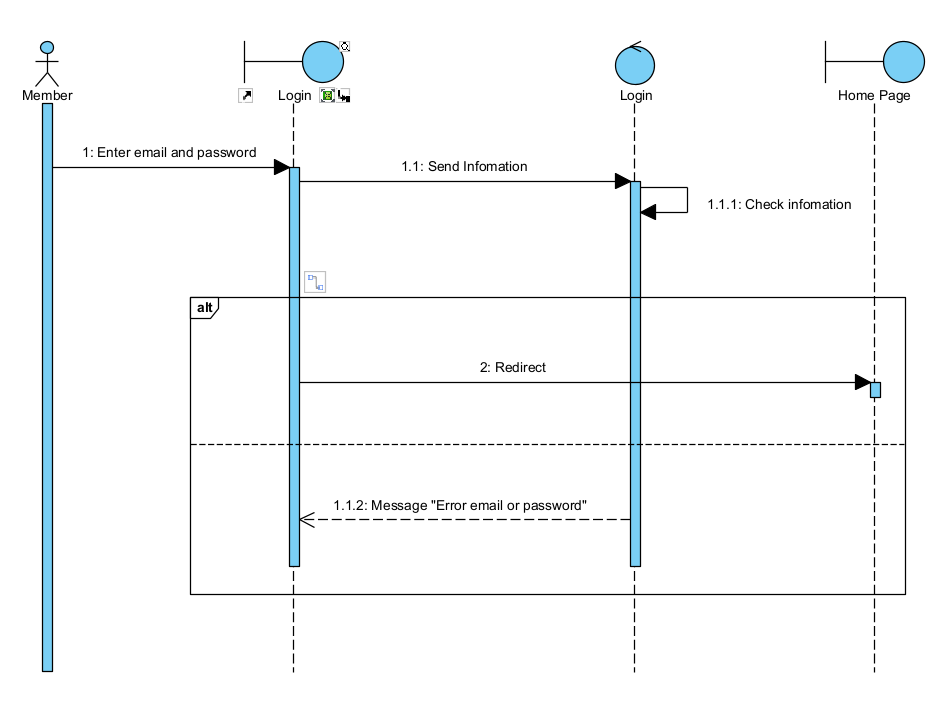
\includegraphics[width=0.8\linewidth]{figures/sequences/sequence-login.png}
        \caption{Biểu đồ Sequence Đăng nhập}
    \end{figure}

    \subsection{Biểu đồ Sequence Cập nhật thông tin người dùng}
    \begin{figure}[H]
        \centering
        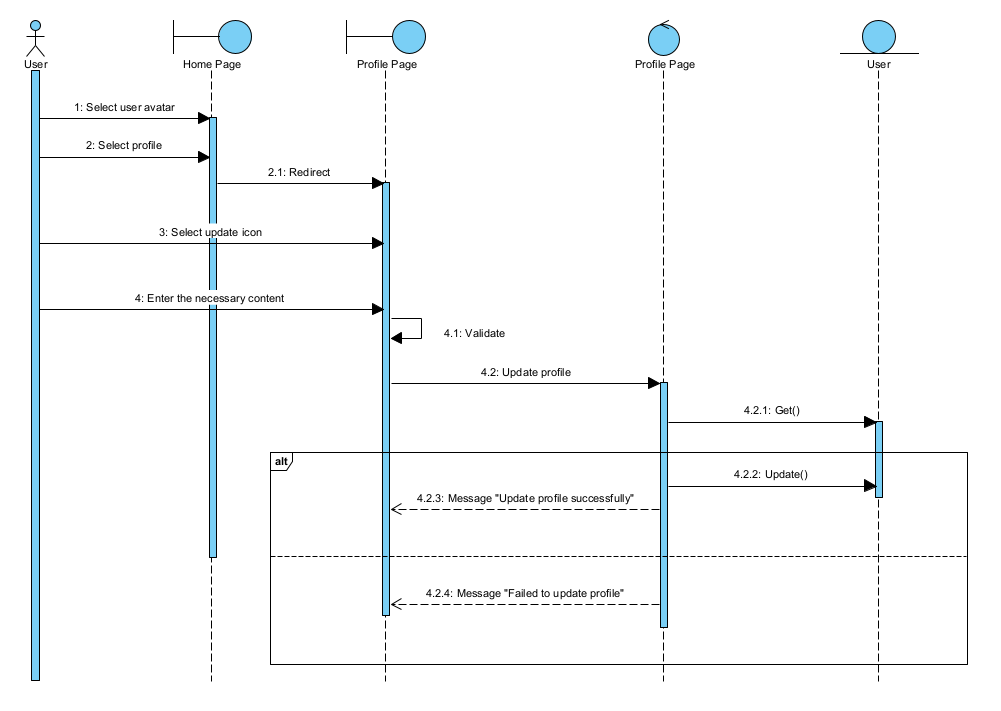
\includegraphics[width=0.8\linewidth]{figures/sequences/sequence-update-user.png}
        \caption{Biểu đồ Sequence Cập nhật thông tin người dùng}
    \end{figure}

    \subsection{Biểu đồ Sequence Tạo bài viết}
    \begin{figure}[H]
        \centering
        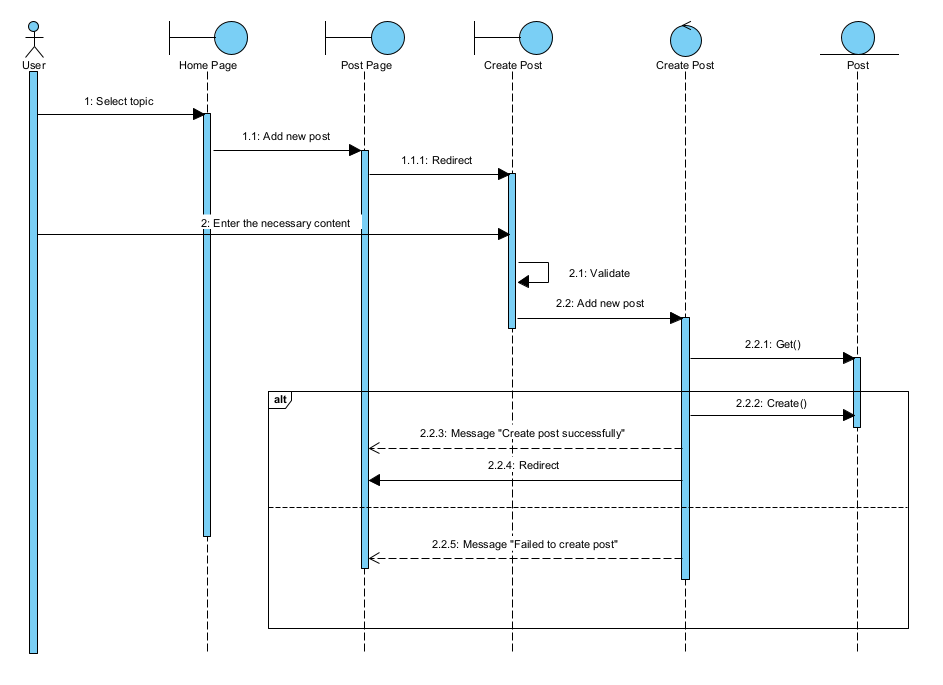
\includegraphics[width=0.8\linewidth]{figures/sequences/sequence-post-create.png}
        \caption{Biểu đồ Sequence Tạo bài viết}
    \end{figure}

    \subsection{Biểu đồ Sequence Tạo bình luận}
    \begin{figure}[H]
        \centering
        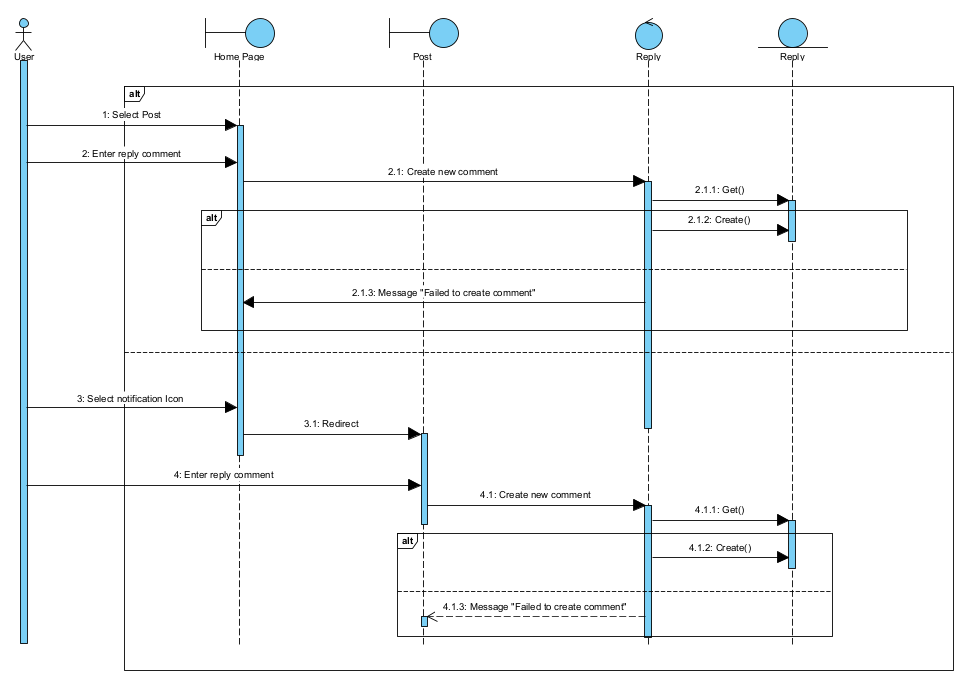
\includegraphics[width=0.8\linewidth]{figures/sequences/sequence-reply.png}
        \caption{Biểu đồ Sequence Tạo bình luận}
    \end{figure}

    \subsection{Biểu đồ Sequence Tạo vai trò}
    \begin{figure}[H]
        \centering
        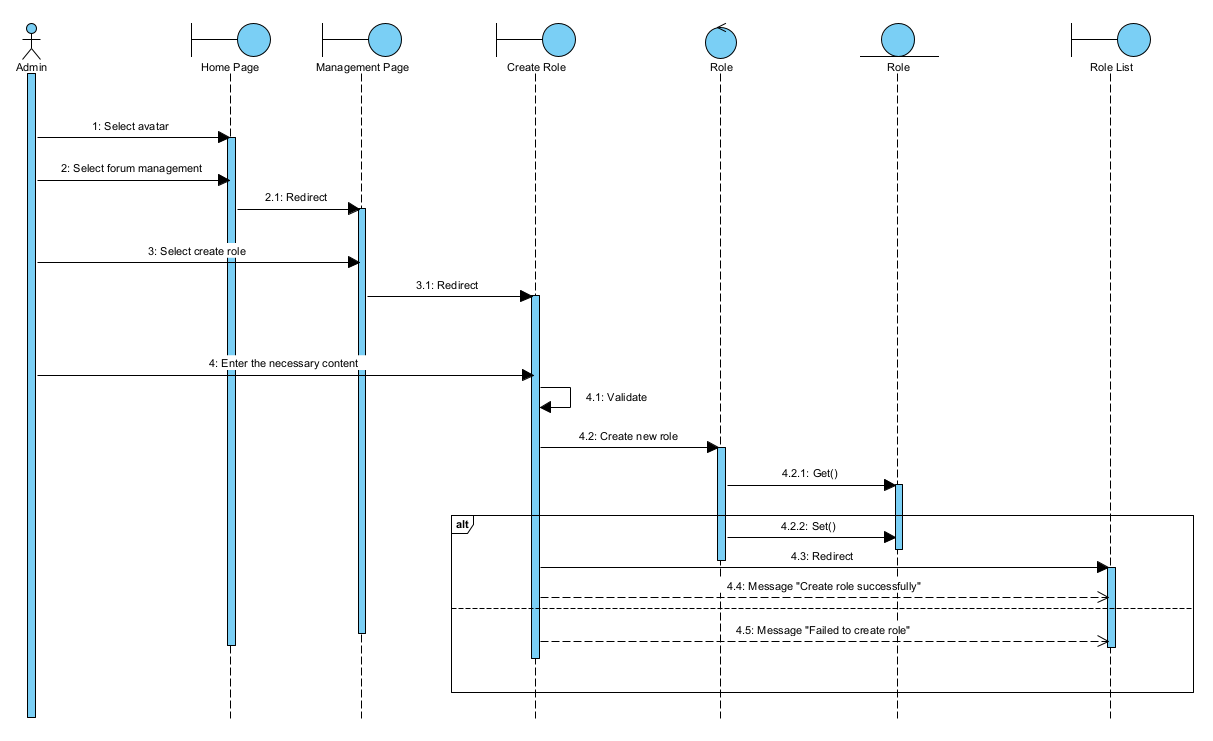
\includegraphics[width=0.8\linewidth]{figures/sequences/sequence-role-create.png}
        \caption{Biểu đồ Sequence Tạo vai trò}
    \end{figure}

    \subsection{Biểu đồ Sequence Gán vai trò cho người dùng}
    \begin{figure}[H]
        \centering
        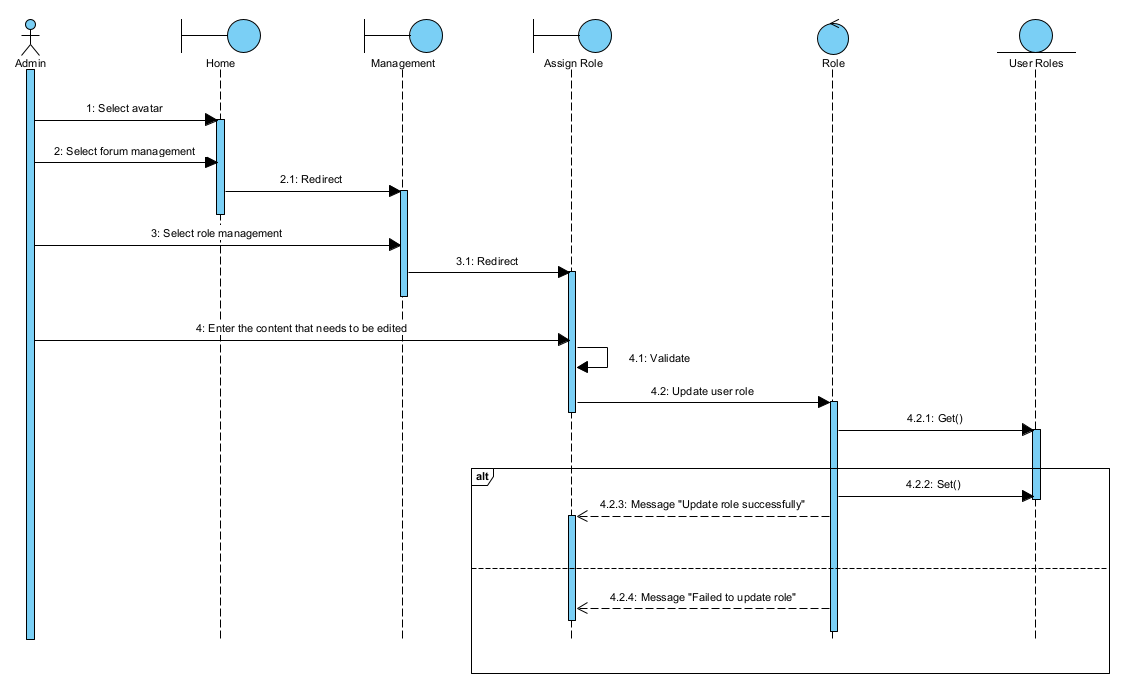
\includegraphics[width=0.8\linewidth]{figures/sequences/sequence-role-assign.png}
        \caption{Biểu đồ Sequence Gán vai trò cho người dùng}
    \end{figure}
\end{document}